\chapter{Related software frameworks and libraries}\label{chap:related-software-frameworks-and-libraries}

\section*{}

Cooperative assembly of objects by robots is a multidisciplinary problem that requires advanced computer software systems. In order to speed up the implementation and deployment of the assembly system, several frameworks and libraries will be used. Among the most important are the \gls{ros} for the system architecture, Gazebo for simulation and testing, \gls{opencv} / \gls{pcl} for 2D / 3D perception and the RoboEarth / RoboHow projects software for robotics cognition.




\section{Software frameworks}

FF

\subsection{\glsentrytext{ros}}

\begin{wrapfigure}{r}{0.23\textwidth}
	\centering
	\vspace*{-2em}
	\includegraphics*[width=0.88\textwidth]{software/ros-logo}
	\caption{\glsentrytext{ros} logo}
	\label{fig:ros-logo}
\end{wrapfigure}

\gls{ros}\footnote{\url{http://www.ros.org}} \cite{Quigley2009} is a software framework designed to ease the development of robot systems. It provides seamless integration between hardware drivers and software modules, allowing a fast transition between simulation and deployment. It's an open source project that offers a distributed computing framework with several core libraries and development tools that aims to speedup software prototyping, testing and deployment.

The \gls{ros} architecture was designed from the beginning to be a distributed peer-to-peer software framework that could be deployed in several operating systems and implemented in a range of different programming languages. However, given that most of the \gls{ros} community prefers open source software, the Ubuntu\footnote{\url{http://www.ubuntu.com}} operating system is the main developing and testing environment, and as such, the recommended choice for \gls{ros} developers. Moreover, considering that robotics research requires software with both performance and maintainability at its core, the C++\footnote{\url{http://www.cplusplus.com}} programming language is used in most of the available packages, along with Python\footnote{\url{https://www.python.org}} and Java\footnote{\url{https://www.java.com}}.

Being a distributed computing framework, \gls{ros} relies in network connections and exchange of messages to perform the intended tasks. As such, its architecture was developed to follow a publish / subscribe pattern (\gls{ros} topics\footnote{\url{http://wiki.ros.org/Topics}}) and request and reply communication paradigm (\gls{ros} services\footnote{\url{http://wiki.ros.org/Services}} and actions\footnote{\url{http://wiki.ros.org/actionlib}}). This allows \gls{ros} nodes\footnote{\url{http://wiki.ros.org/Nodes}} (operating system processes) to be deployed in different computing platforms with ease and simplifies testing and exchange of software modules.


\subsection{Orocos}

\begin{wrapfigure}{r}{0.23\textwidth}
	\centering
	\vspace*{-2em}
	\includegraphics*[width=0.52\textwidth]{software/orocos-logo}
	\caption{Orocos project logo}
	\label{fig:orocos-logo}
\end{wrapfigure}

The \gls{orocos}\footnote{\url{http://www.orocos.org/}} is a real-time robot control framework with a set of software libraries for managing forward / inverse robot arm kinematics, data filtering (Dynamic Bayesian Networks, Kalman filters, particle filters) and robot arm motion control using the \gls{itasc}.




\section{Knowledge management and reasoning libraries}

FF

\subsection{RoboEarth}

\begin{wrapfigure}{r}{0.23\textwidth}
	\centering
	\vspace*{-2em}
	\includegraphics*[width=0.9\textwidth]{software/robo-earth-logo}
	\caption{RoboEarth logo}
	\label{fig:robo-earth-logo}
\end{wrapfigure}

During the RoboEarth\footnote{\url{http://roboearth.org}} project it was developed a set of modular software components that enabled robots to share reusable knowledge and offload heavy computation tasks to the cloud. In \cref{fig:robo-earth-software-interaction,fig:robo-earth-software-overview} it is given a brief overview of the main software modules of the RoboEarth project that will be presented in the next sections.


\begin{figure}[H]
	\begin{floatrow}[2]
		\ffigbox[\FBwidth]
		{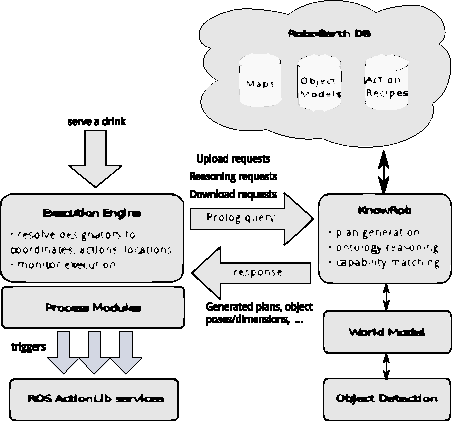
\includegraphics[height=.35\textheight]{software/robo-earth-software-interaction}}
		{\caption[Interaction between the RoboEarth software modules]{Interaction between the RoboEarth software modules \cite{DiMarco2013}}\label{fig:robo-earth-software-interaction}}

		\ffigbox[\FBwidth]
		{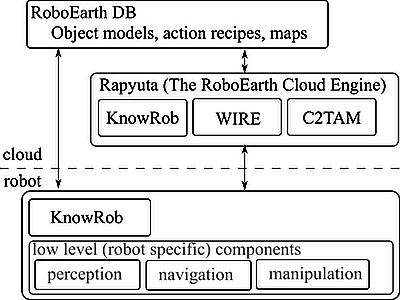
\includegraphics[height=.19\textheight]{software/robo-earth-software-overview}}
		{\caption[Overview of the RoboEarth main software modules]{Overview of the RoboEarth main software modules\protect\footnotemark}\label{fig:robo-earth-software-overview}}
	\end{floatrow}
\end{figure}
\footnotetext{\url{http://roboearth.org/software-components}}


\subsection{KnowRob}

KnowRob\footnote{\url{http://www.knowrob.org}} \cite{tenorth2011PhD,Tenorth2013k} is a knowledge processing framework that combines world representation using ontologies with a Prolog reasoning engine in order to semantic learn new reusable skills from different data sources. It has integrated several reasoning, perception and human-machine interaction software packages\footnote{\url{http://wiki.ros.org/knowrob}} that allow to semantically analyze \gls{cad} models \cite{Lavoue2005,Tenorth2013cad}, visually edit robot tasks\footnote{\url{http://www.knowrob.org/doc/action_recipe_editor}} and semantic environment maps\footnote{\url{http://www.knowrob.org/doc/semantic_map_editor}} \cite{Pangercic2012} and also perform robot motions\footnote{\url{http://knowrob.org/doc/motion_constraints}} \cite{tenorth14motiontemplates} based on the semantic knowledge of the objects and the environment.


\subsection{RoboHow}

\begin{wrapfigure}{r}{0.23\textwidth}
	\centering
	\vspace*{-2em}
	\includegraphics*[width=0.9\textwidth]{software/robo-how-logo}
	\caption{RoboHow logo}
	\label{fig:robo-how-logo}
\end{wrapfigure}

The RoboHow project\footnote{\url{https://robohow.eu}} continued the development of the RoboEarth research and added several new software packages targeted at service robotics and knowledge extraction. The next sections present the main software modules developed during this project.


\subsection{\glsentrytext{openease}}

%\vspace*{-1cm}
\begin{wrapfigure}{r}{0.23\textwidth}
	\centering
	\vspace*{-2em}
	\includegraphics*[width=0.75\textwidth]{software/open-ease-logo}
	\caption{\glsentrytext{openease} logo}
	\label{fig:open-ease}
\end{wrapfigure}

The \gls{openease}\footnote{\url{http://www.open-ease.org}} \cite{Beetz2015} is a remote knowledge representation and processing service built on top of KnowRob\footnote{\url{http://www.knowrob.org}} and \gls{ros} that allows to interpret, analyze, visualize and learn from experience and demonstration.


\subsection{OpenCyc}

\begin{wrapfigure}{r}{0.23\textwidth}
	\centering
	\vspace*{-2em}
	\includegraphics*[width=0.7\textwidth]{software/open-cyc-logo}
	\caption{OpenCyc logo}
	\label{fig:open-cyc}
\end{wrapfigure}

OpenCyc\footnote{\url{http://www.cyc.com/platform/opencyc}} is a reasoning engine with a large ontology and knowledge base that is capable of extracting semantic information from natural language. It also has \gls{ai} capabilities which make it suitable for implementing domain-specific expert systems and game \glspl{ai}.


\section{Collision detection / physics engines}

- fcl
- Bullet
- ODE
- Simbody
- Dart


\section{Control and manipulation libraries}

FF

\subsection{OMPL}

Open Motion Planning Library


\subsection{MoveIt!}

FF


\subsection{GraspIt!}

FF


\subsection{Robotics Library}

\begin{wrapfigure}{r}{0.23\textwidth}
	\centering
	\vspace*{-2em}
	\includegraphics*[width=0.99\textwidth]{software/robotics-library-logo}
	\caption{Robotics Library logo}
	\label{fig:robotics-library-logo}
\end{wrapfigure}

The Robotics Library\footnote{\url{http://www.roboticslibrary.org}} provides a set of C++ software libraries for managing robot arm kinematics, motion control, collision detection, path planing and visual inspection.


\subsection{\glsentrytext{cram}}

The \gls{cram}\footnote{\url{http://www.cram-system.org/cram}} \cite{Beetz2010} is a software toolbox that allows to perform complex object manipulation tasks using flexible specification of reactive robot motion control plans using Common Lisp. In \cref{fig:cram-overview} it is shown the integration with the KnowRob for logic reasoning and semantic cognition.

\begin{figure}[H]
	\centering
	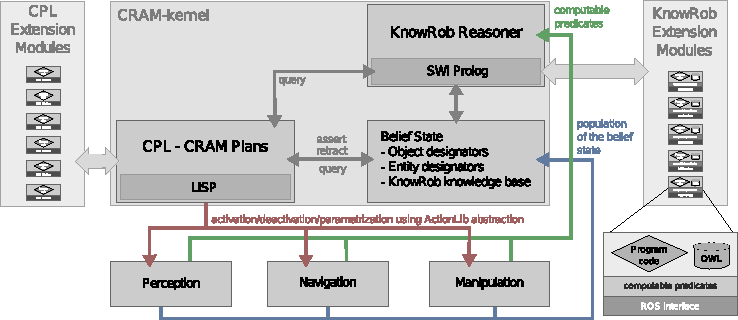
\includegraphics[width=0.62\linewidth]{software/cram-overview}
	\caption{Overview of the \glsentrytext{cram} main software modules}
	\label{fig:cram-overview}
\end{figure}


\subsection{\glsentrytext{itasc}}

The \gls{itasc}\footnote{\url{http://www.orocos.org/wiki/orocos/itasc-wiki}} \cite{DeSchutter-ijrr2007} is a software framework for generation of robot motions by specifying constraints between the objects, the robots and the environment. In \cref{fig:itasc-overview} it is presented an overview of the \gls{itasc} main software modules.

\begin{figure}[H]
	\centering
	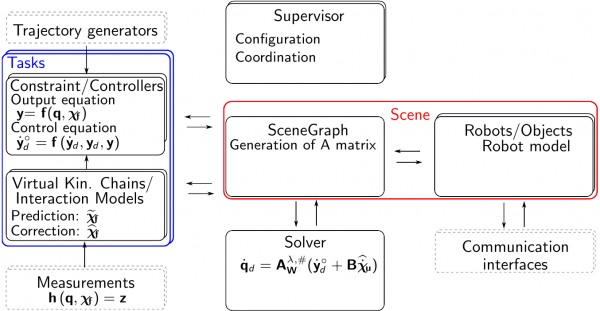
\includegraphics[width=0.56\linewidth]{software/itasc-overview}
	\caption[Overview of the \glsentrytext{itasc} framework]{Overview of the \glsentrytext{itasc} framework\protect\footnotemark}
	\label{fig:itasc-overview}
\end{figure}
\footnotetext{\url{http://www.orocos.org/wiki/orocos/itasc-wiki/2-itasc-software}}




\section{Perception libraries}

FF

\subsection{\glsentrytext{pcl}}

\begin{wrapfigure}{r}{0.23\textwidth}
	\centering
	\vspace*{-2em}
	\includegraphics*[width=0.88\textwidth]{software/pcl-logo}
	\caption{\glsentrytext{pcl} logo}
	\label{pcl-logo}
\end{wrapfigure}

\gls{pcl}\footnote{\url{http://pointclouds.org}} \cite{Rusu2011} is an open source project that provides algorithms for 3D perception. These algorithms can be used to filter and register point clouds as well as perform object segmentation, recognition and tracking. In \Cref{fig:pcl-dependency-graph} it is presented an overview of the main modules currently available in \gls{pcl}.

\begin{figure}[H]
	\centering
	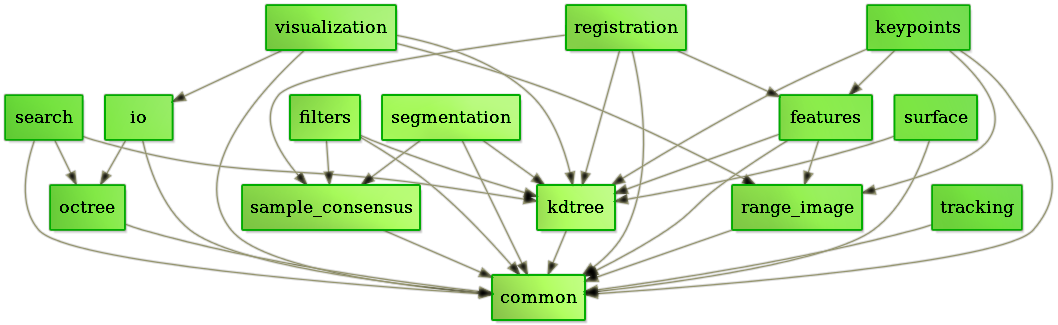
\includegraphics[width=.7\textwidth]{software/pcl-dependency-graph}
	\caption[\glsentrydesc{pcl}]{\glsentrydesc{pcl}\protect\footnotemark}
	\label{fig:pcl-dependency-graph}
\end{figure}
\footnotetext{\url{http://pointclouds.org/about}}


\subsection{\glsentrytext{opencv}}

\begin{wrapfigure}{r}{0.23\textwidth}
	\centering
	\vspace*{-2em}
	\includegraphics*[width=0.6\textwidth]{software/opencv-logo}
	\caption{\glsentrytext{opencv} logo}
	\label{fig:opencv-logo}
\end{wrapfigure}

\gls{opencv}\footnote{\url{http://opencv.org}} provides a wide range of state of the art algorithms for processing image sensor data, from segmentation and object quality analysis to advanced object recognition using feature matching or machine learning. It also provides a set of modules for extracting 3D geometry using structured light or stereo vision methods along with image stitching, video stabilization, face / marker detection, among many others.


\subsection{WIRE}

The \gls{wire}\footnote{\url{http://wiki.ros.org/wire}} \cite{Elfring2013} is a probabilistic multi-object tracking system capable of maintaining a consistent world state of detected objects even when they are outside of the robot observable area or are partially occluded.


\subsection{C2TAM}

The \gls{c2tam}\footnote{\url{https://sites.google.com/site/c2tamvisualslam}} \cite{Riazuelo2014} is a remote and cooperative visual \gls{slam} system capable of estimating the robots cameras pose in the world while creating a consistent map of the environment using image feature matching and loop closing techniques. Other related work developed within the RoboEarth project includes the semantic mapping of the environment \cite{Riazuelo2015} and also the low cost mapping systems \cite{Mohanarajah2015}.


\subsection{FORTH 3D Hand Tracking library}

The FORTH 3D Hand Tracking Library\footnote{\url{http://cvrlcode.ics.forth.gr/handtracking}} \cite{Oikonomidis2011,Kyriazis2012} provides an accurate and real-time approach (relying on \gls{gpu} acceleration) for tracking the 3D pose and orientation of the hand fingers of a person (26 degrees of freedom) using an RGB-D sensor.


\subsection{Rapyuta}

Rapyuta\footnote{\url{http://rapyuta.org}} \cite{Hunziker2013} is a \gls{paas} computing environment built on top of \gls{ros} that allows to offload heavy computation tasks (such as environment mapping, object recognition, machine learning, among others) from the robot's embedded systems to the cloud.




\section{Simulators}

FF

\subsection{Gazebo}

\begin{wrapfigure}{r}{0.23\textwidth}
	\centering
	\vspace*{-2em}
	\includegraphics*[width=0.88\textwidth]{software/gazebo-logo}
	\caption{Gazebo logo}
	\label{fig:gazebo-logo}
\end{wrapfigure}


Gazebo\footnote{\url{http://gazebosim.org}} is a 3D multi-robot simulator capable of generating hardware sensor data for different kinds of robots while providing a realistic environment with physics simulation and 3D visualization. It is very useful to speedup testing of algorithms with different types of robots and environments. In \Cref{fig:gazebo-ros-integration} it is shown how Gazebo can be used instead of a real robot, without requiring any implementation code modification (because it implements the same \gls{ros} interfaces that the hardware drivers use).

\begin{figure}[H]
	\centering
	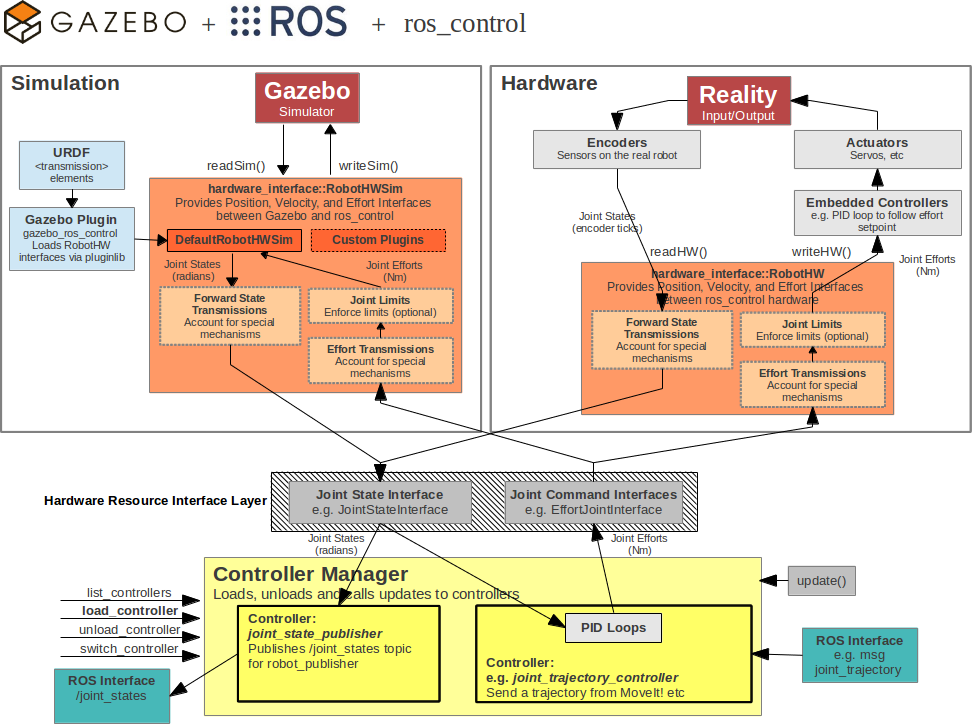
\includegraphics[width=.9\textwidth]{software/gazebo-ros-integration}
	\caption[Integration of \glsentrytext{ros} and Gazebo]{Integration of \glsentrytext{ros} and Gazebo\protect\footnotemark}
	\label{fig:gazebo-ros-integration}
\end{figure}
\footnotetext{\url{http://gazebosim.org/tutorials?tut=ros_control}}


\subsection{RoboDK}

\begin{wrapfigure}{r}{0.23\textwidth}
	\centering
	\vspace*{-2em}
	\includegraphics*[width=0.9\textwidth]{software/robodk-logo}
	\caption{RoboDK logo}
	\label{fig:robodk-logo}
\end{wrapfigure}

The \gls{robodk} \footnote{\url{https://www.robodk.com}} is a 3D simulator and an offline programming environment for industrial robots with and extended library of robotic arms and is capable of \gls{gui} / script specification of robot motions with support for 2D / 3D visualization / inspection.
